\documentclass{article}
\usepackage{ctex}
\usepackage{array}
\usepackage{fontspec}
\usepackage{multirow}
\usepackage{multicol}
\usepackage{geometry}
\usepackage{lastpage}
\usepackage{titlesec}
\usepackage[shortlabels]{enumitem}
\linespread{1.287}
\geometry{left=3.18cm,right=3.18cm,top=2.54cm,bottom=2.54cm}
\setlist[enumerate]{nosep}
\begin{document}
\newpagestyle{main}{
    \sethead{\ContestName}{}{\ContestType \ContestDate}
    \setfoot{}{第\thepage{}页共\pageref{LastPage} 页}{}
    \headrule
}
\pagestyle{main}
\protected\def\pdfliteral{\pdfextension literal}
\newcommand{\BoldAsWord}[1]{{\pdfliteral{2 Tr 0.2857 w}#1\pdfliteral{0 Tr}}}
\newcommand{\SlantAsWord}[1]{{\pdfliteral{1 0 0.3333 1 0 0 cm}#1\pdfliteral{1 0 -0.3333 1 0 0 cm}}}
\newcommand{\hei}[1]{{\fontspec{SimHei}{#1}}}
\newcommand{\kai}[1]{{\fontspec{KaiTi_GB2312}{#1}}}
\newcommand{\tnr}[1]{{\fontspec{Times New Roman}{#1}}}
\newcommand{\cn}[1]{{\fontspec{Courier New}{#1}}}
\setmainfont{Times New Roman}
% Contest Settings for NOIp
\newcommand{\ContestName}{NOIp模拟题}
\newcommand{\ContestType}{提高组}
\newcommand{\ContestDate}{day1}
\newcommand{\ChineseNameA}{魔法少女技能测试}
\newcommand{\ChineseNameB}{特别的樱花树}
\newcommand{\ChineseNameC}{特奥多尔不是骗子!}
\newcommand{\EnglishNameA}{shoujoo}
\newcommand{\EnglishNameB}{sakura}
\newcommand{\EnglishNameC}{teodor}
\newcommand{\TimeLimitA}{1}
\newcommand{\TimeLimitB}{1}
\newcommand{\TimeLimitC}{1}
\newcommand{\TestPtsNumA}{100}
\newcommand{\TestPtsNumB}{100}
\newcommand{\TestPtsNumC}{100}
\newcommand{\TestPtsScoA}{1}
\newcommand{\TestPtsScoB}{1}
\newcommand{\TestPtsScoC}{1}
\newcommand{\AddiSampleA}{有}
\newcommand{\AddiSampleB}{有}
\newcommand{\AddiSampleC}{有}
\newcommand{\CheckMethod}{全文比较模式(忽略行尾多余的空格和制表符)}
\newcommand{\ProblemTypeA}{传统}
\newcommand{\ProblemTypeB}{传统}
\newcommand{\ProblemTypeC}{传统}
\newcommand{\MemoryLimitA}{256}
\newcommand{\MemoryLimitB}{256}
\newcommand{\MemoryLimitC}{256}
\newcommand{\Notice}{\begin{enumerate}
\item{\textbf{请特别注意,若选择在NOI Linux下评测,则需要按照NOI Linux的要求建立题目子文件夹;若选择在lemon下评测,则无需建立题目子文件夹。}}
\item{我已经不会判断题目难度了,所以题目难度与题号无关,但是第一题应该是最简单的了。}
\item{题目难度不大,希望你们都能拿到一半以上(150分以上)的分数。}
\item{祝大家好运。\textbf{别忘记开文件!别忘记开文件!别忘记开文件!别写错文件名!别写错文件名!别写错文件名!重要的事情说三遍!!!}}
\end{enumerate}}
\newcommand{\ProblemDescribeA}{你在一个$H$行$W$列的网格上,我们规定在第$i$行第$j$列的格子记作格子$(i,j)$。
网格中的每个格子都有一个编号,自左向右自上而下为$1$到$H\times W$,每个格子上的数记作$A_{i,j}$。

你作为一个魔法少女,可以通过消耗$|x-i|+|y-j|$点魔法点从格子$(i,j)$传送到格子$(x,y)$。

你现在要进行$Q$次魔法测验来证明你作为魔法少女的能力。

第$i$轮测试将按以下流程进行:
\begin{itemize}
\item{测试的开始,你在写有$L_i$的格子的位置。}
\item{令$x$为所在格子上的数,你要跳到写有$(x+d)$的格子上,重复这一流程,直到你跳到写有$R_i$的格子上,测试结束。}
\end{itemize}

对于每一次测试,计算测试需要消耗的魔法点数。}
\newcommand{\InputStyleA}{输入文件格式如下:

$H\ W\ D$\par
$A_{1,1}\ A_{1,2}\ \cdots\ A_{1,W}$\par
$\ \vdots$\par
$A_{H,1}\ A_{H,2}\ \cdots\ A_{H,W}$\par
$Q$\par
$L_1\ R_1$\par
$\ \vdots$\par
$L_Q\ R_Q$\par
}
\newcommand{\OutputStyleA}{对于每一组测试,输出测试需要消耗的魔法点数。

输出应该按照输入的顺序。}
\newcommand{\SampleInputA}{
3 3 2\par
1 4 3\par
2 5 7\par
8 9 6\par
1\par
4 8\par}
\newcommand{\SampleOutputA}{
5\par}
\newcommand{\SampleExplainationA}{
网格的布局如下:
\begin{center}
\begin{tabular}{|c|c|c|}
\hline
1&4&3\\
\hline
2&5&7\\
\hline
8&9&6\\
\hline
\end{tabular}
\end{center}
\begin{itemize}
\item{格子$(1,2)$上的数为$4$。}
\item{格子$(3,3)$上的数为$6$。}
\item{格子$(3,1)$上的数为$8$。}
\end{itemize}
最初少女在格子$(1,2)$上,格子上的数为$4$,然后她会直接传送到格子上的数为$6$的格子,即格子$(3,3)$上,然后传送到格子$(3,1)$上,格子上的数为$8$,等于$R_i$了,测试结束。

因此,第一次测试消耗的魔法点数为$(|3-1|+|3-2|)+(|3-3|+|1-3|)=5$。}
\newcommand{\DataSizeA}{对于30\%的数据,$1\le H,W\le 50,Q\le 10000$;

对于另外30\%的数据,$1\le H,W\le 100,Q\le 5000$;

对于100\%的数据:$1\le D\le H\times W,1\le A_{i,j}\le H\times W,A_{i,j}\neq A_{x,y((i,j)\neq (x,y))},1\le Q\le 10^5,1\le L_i\le R_i\le H\times W$。

数据保证$(R_i-L_i)$是$D$的一个倍数(如果不能理解这句话,可以认为数据保证对于每组测试测试一定有解,即不存在跳不到$R_i$这个格子的情况)。
}

\newcommand{\ProblemDescribeB}{幻想乡的花园里生长着一棵特别的樱花树,每年开一次花。它的特别之处可以用下列方法来解释:它有$n$个花苞,编号为$1$到$n$。编号为$1$的花苞在树根上,其它所有编号为$i(i>1)$的花苞位于编号为第$p_i$个花苞上方,它们之间有一根树枝相连。

一旦这棵树开始开花,每一个花苞都会开出一朵花。在花出现的同时,它们开始沿着树枝向下滚,直到滚到树枝上停下。在每一秒内,除了在树根上的樱花以外,其它所有樱花都同时向下滚$1$个树枝的距离。例如位于第$a$个花苞位置的花到达第$p_a$个花苞的位置。在树根处的花会在同时被阿卡迪摘下。这棵树的第二个特别之处在于一旦两朵花落在同一个花苞上它们就会\textbf{消失}。这样的事发生在每一对花上,例如如果在同一个花苞上同时有$5$朵花,这个花苞上只会剩下$1$朵花;如果有$8$朵花,所有的花都会消失。因此,每个花苞中不会同时有多于$1$朵花。

你需要帮助阿卡迪数算出一次收获她能从树根上摘下来多少朵花。}
\newcommand{\InputStyleB}{输入的第一行仅包含一个整数$n$,表示花苞的数量。

输入的第二行包含一个$(n-1)$个数的序列$p_2,p_3,\ldots,p_n(1\le p_i\le i)$,$p_i$是编号为$i$的花苞会滚到的花苞编号。}
\newcommand{\OutputStyleB}{输出仅包含一行一个整数,表示阿卡迪一次收获能够在$1$号花苞摘到多少朵花。}
\newcommand{\SampleInputB}{18\par
1 1 1 4 4 3 2 2 2 10 8 9 9 9 10 10 4\par}
\newcommand{\SampleOutputB}{4\par}
\newcommand{\SampleExplainationB}{阿卡迪能摘到$3$朵花,第一朵花是开始在树根的花。在一秒内,$2$号花苞内的花会滚到$1$号花苞中(阿卡迪会摘下它),同时,来自$3$、$4$、$5$号花苞的花会滚到$2$号花苞中。其中两个会消失,剩下的$1$个会在下一秒滚到$1$号花苞,阿卡迪会摘下它。

下图所示为这棵树的初始形态:
\begin{center}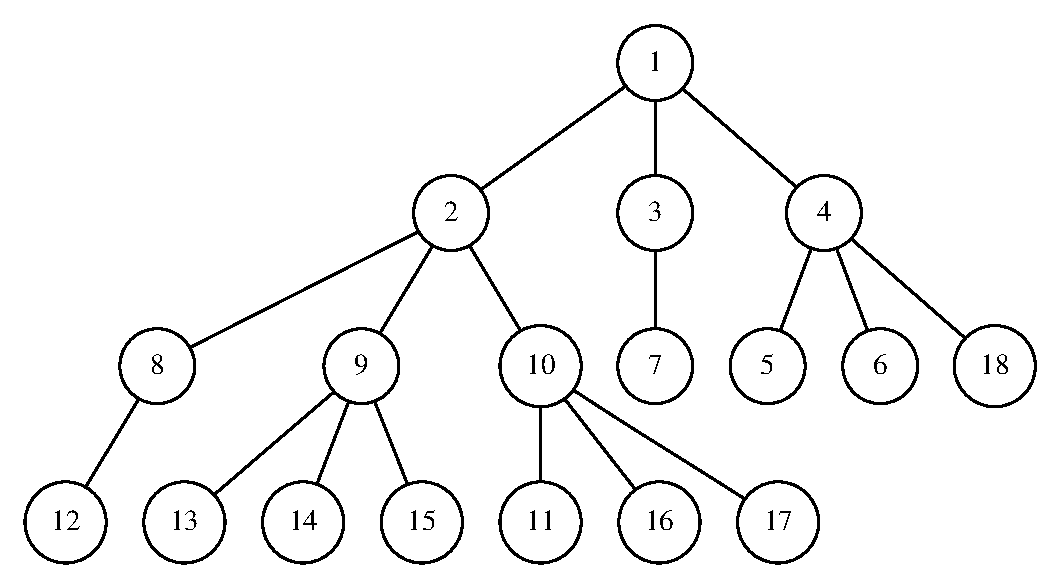
\includegraphics[width=8cm]{graph1.eps}\end{center}}
\newcommand{\DataSizeB}{对于30\%的数据,$2\le n\le 10$;

对于60\%的数据,$2\le n\le 1000$;

对于所有数据,$2\le n\le 100\,000$。}

\newcommand{\ProblemDescribeC}{年轻的特奥多尔喜欢画画。他最喜欢的事情就是在区间$[1,n]$内画线段。有一天,特奥多尔注意到他刚画的图具有一个有趣的特性:不存在一个整数点,被他画的图上的每一条线段所覆盖。发现了这个事实后,特奥多尔决定把这个事实分享给萨沙。

萨沙知道特奥多尔喜欢炫耀,所以她从不信任他。特奥多尔想证明自己有的时候也是可以被信任的,所以他决定向萨沙保证他的图片里没有整数点被所有的线段覆盖。然而特奥多尔很懒,他既不会告诉萨沙线段的端点,也不会告诉她线段的数量。所以特奥多尔建议萨沙向他问一系列类似于“特奥多尔的画中有多少条线段覆盖了给定整数点$x_i$?”的问题,保证特奥多尔给出的答案是正确的。

两个人都忙于学习并且没有太多时间,所以他们向你询问萨沙在知道特奥多尔是不是撒谎之前,最多能向特奥多尔提问多少次。

需要注意的是萨沙不知道特奥多尔的图画里的线段的数量。显然,萨沙是个聪明人,她不会重复询问同一个点。}
\newcommand{\InputStyleC}{输入的第一行包含两个整数$n$和$m$,表示特奥多尔的图画中的线段数和萨沙可以提问的最大次数。

接下来的$n$行,第$i$行包含两个整数$l_i$和$r_i$,表示图画中第$i$条线段的左右端点。需要注意的是线段的左右端点可能为同一个点。

数据保证没有整数点被所有线段覆盖。}
\newcommand{\OutputStyleC}{输出仅包含一行,一个整数$k$表示最大的集合$(x_i,cnt(x_i))$的大小(注意是数学集合的概念,集合中的元素具有互异性)。其中$1\leq x_i\le m$,且$cnt(x_i)$是覆盖端点$x_i$的线段的数量,使得一个人在只知道这个集合并且不知道$n$的情况下,不能确定是否存在一个点被图画中的所有线段覆盖。}
\newcommand{\SampleInputC}{4 6\par
1 3\par
2 3\par
4 6\par
5 6\par}
\newcommand{\SampleOutputC}{5\par}
\newcommand{\SampleExplainationC}{样例中萨沙在询问$5$个点如$1,2,3,5,6$后,仍然不能确定特奥多尔是不是对她撒了谎。但是一旦她获得了区间$[1,6]$内每个整数点的信息,她就能确定特奥多尔没有对她撒谎。}
\newcommand{\DataSizeC}{对于30\%的数据,$1\le n,m\le 100$;

对于100\%的数据,$1\le n,m\le 100\, 000$。

数据还保证$1\le l_i\le r_i\le m$。}

\begin{center}\zihao{3}{\textbf{\ContestName}}\end{center}
\begin{center}\zihao{-1}{\heiti{\ContestType\hspace{1em}\hei{\ContestDate}}}\end{center}
\begin{center}\zihao{4}{\kaishu{\BoldAsWord{(请选手务必仔细阅读本页内容)}}}\end{center}
\ \par
\zihao{5}
\noindent\vspace{0.5pt}\hspace{-1em}\BoldAsWord{一.题目概况}\par
\noindent
\makebox[\linewidth][c]{
\begin{tabular}{|m{3.69cm}<{\centering}|m{3.69cm}<{\centering}|m{3.69cm}<{\centering}|m{3.69cm}<{\centering}|}
\hline
中文题目名称&\ChineseNameA&\ChineseNameB&\ChineseNameC\\
\hline
英文题目与子目录名&\EnglishNameA&\EnglishNameB&\EnglishNameC\\
\hline
可执行文件名&\EnglishNameA&\EnglishNameB&\EnglishNameC\\
\hline
输入文件名&\EnglishNameA.in&\EnglishNameB.in&\EnglishNameC.in\\
\hline
输出文件名&\EnglishNameA.out&\EnglishNameB.out&\EnglishNameC.out\\
\hline
每个测试点时限&\TimeLimitA 秒&\TimeLimitB 秒&\TimeLimitC 秒\\
\hline
测试点数目&\TestPtsNumA&\TestPtsNumB&\TestPtsNumC\\
\hline
每个测试点分值&\TestPtsScoA&\TestPtsScoB&\TestPtsScoC\\
\hline
附加样例文件&\AddiSampleA&\AddiSampleB&\AddiSampleC\\
\hline
结果比较方式&\multicolumn{3}{c|}{\CheckMethod}\\
\hline
题目类型&\ProblemTypeA&\ProblemTypeB&\ProblemTypeC\\
\hline
运行内存上限&\MemoryLimitA M&\MemoryLimitB M&\MemoryLimitC M\\
\hline
\end{tabular}
}
 \par
\noindent\vspace{0.5pt}\hspace{-1em}\BoldAsWord{二.提交源程序文件名}

\noindent
\makebox[\linewidth][c]{
\begin{tabular}{|m{3.69cm}<{\centering}|m{3.69cm}<{\centering}|m{3.69cm}<{\centering}|m{3.69cm}<{\centering}|}
\hline
对于C++语言&\EnglishNameA.cpp&\EnglishNameB.cpp&\EnglishNameC.cpp\\
\hline
对于C语言&\EnglishNameA.c&\EnglishNameB.c&\EnglishNameC.c\\
\hline
对于Pascal语言&\EnglishNameA.pas&\EnglishNameB.pas&\EnglishNameC.pas\\
\hline
\end{tabular}
}
 \par
\noindent\vspace{0.5pt}\hspace{-1em}\BoldAsWord{三.编译命令(不包含任何优化开关)}

\noindent
\makebox[\linewidth][c]{
\begin{tabular}{|m{3.69cm}<{\centering}|m{3.69cm}<{\centering}|m{3.69cm}<{\centering}|m{3.69cm}<{\centering}|}
\hline
对于C++语言&g++ -o \EnglishNameA\ \EnglishNameA.cpp -lm&g++ -o \EnglishNameB\ \EnglishNameB.cpp -lm&g++ -o \EnglishNameC\ \EnglishNameC.cpp -lm\\
\hline
对于C语言&gcc -o \EnglishNameA\ \EnglishNameA.cpp -lm&gcc -o \EnglishNameB\ \EnglishNameB.cpp -lm&gcc -o \EnglishNameC\ \EnglishNameC.cpp -lm\\
\hline
对于Pascal语言&fpc \EnglishNameA.pas&fpc \EnglishNameB.pas&fpc \EnglishNameC.pas\\
\hline
\end{tabular}
}
 \par
\noindent\hspace{-1em}\BoldAsWord{注意事项:}\\
\hspace{-1em}\Notice
\newpage
\end{document}